% report.tex — NeurIPS-style submission (use neurips_2021 or later)
\documentclass{article}
\usepackage[preprint]{neurips_2021}
\usepackage{amsmath, amssymb, amsfonts, graphicx, booktabs, hyperref}
\usepackage{microtype}
\usepackage{xcolor}
\title{CS 599: Foundations of Deep Learning --- Assignment \#00001\\
Linear and Logistic Regression using TensorFlow 2 (Eager Execution, No Keras)}
\author{Pavan Prasad Gorintla\\Northern Arizona University}
\date{December 17, 2024}

\begin{document}
\maketitle

\begin{abstract}
This report presents an in-depth implementation of Linear and Logistic Regression models developed using \textbf{TensorFlow~2} in \emph{eager execution} mode, without relying on Keras high-level APIs. For the linear regression task, the model learns the mapping $f(x) = 3x + 2 + \epsilon$ using iterative gradient-based optimisation. We compare several loss functions (L1, L2, Huber, and Hybrid), explore learning rate schedulers, and examine the impact of noise in data, weights, and learning rate. The logistic regression model is evaluated on the Fashion-MNIST dataset to study multi-class classification using manual gradient computation. The project also explores optimiser choice, batch size, overfitting behaviour, and CPU vs GPU training time. Source code and results are available publicly at:  
\textbf{Code Repository:} \\
\url{https://github.com/gorintlapavanprasad/CS599\_DL\_Assignment\_00001}
\end{abstract}

\section{Experimental Setup and Reproducibility}
All experiments are performed in \textbf{TensorFlow~2 (Eager Mode)} with NumPy, Matplotlib, and scikit-learn. Only the TensorFlow dataset loader is used for Fashion-MNIST; no Keras models or layers are employed. Each experiment is conducted with a unique random seed derived by converting the student's first name into a decimal value (\texttt{Pavan} $\to$ 808). Timing is measured on both CPU and GPU to compare computational performance per epoch.

\section{Problem 1: Linear Regression}
\subsection{Model Formulation}
The regression model is defined as $\hat{y} = Wx + b$, optimised using gradient descent computed through \texttt{tf.GradientTape}. Rather than solving analytically, parameters are updated iteratively, giving flexibility to test various learning strategies.

\subsection{Loss Functions}
The following loss formulations were implemented:
\begin{align}
\mathcal{L}_{L2} &= \frac{1}{N}\sum_i (y_i-\hat{y}_i)^2, \quad
\mathcal{L}_{L1} = \frac{1}{N}\sum_i |y_i-\hat{y}_i|, \\
\mathcal{L}_{Huber} &= 
\begin{cases}
\frac{1}{2}(y_i-\hat{y}_i)^2, & |y_i-\hat{y}_i|\le \delta \\
\delta|y_i-\hat{y}_i| - \frac{1}{2}\delta^2, & \text{otherwise}
\end{cases}, \\
\mathcal{L}_{Hybrid} &= \alpha \mathcal{L}_{L1} + (1-\alpha)\mathcal{L}_{L2}.
\end{align}
An additional L2 regularisation term $\lambda(\|W\|_2^2 + \|b\|_2^2)$ is optionally included for better generalisation.

\subsection{Schedulers and Noise}
Learning rate scheduling is studied using:
\begin{enumerate}
    \item \textbf{Plateau-halving:} learning rate is reduced by half when loss stagnates for $p$ epochs.
    \item \textbf{Warmup + Cosine decay:} gradually increases the learning rate at the start, followed by a smooth cosine decay.
\end{enumerate}
Noise is introduced in three forms --- additive data noise, multiplicative weight noise, and random perturbation of the learning rate (LR jitter). These help analyse the model’s stability and robustness to randomness.

\subsection{Key Observations}
\begin{itemize}
    \item \textbf{Loss behaviour:} L2 converges faster for Gaussian noise, while L1 and Huber perform better under outliers or heavy-tailed noise. Hybrid loss ($\alpha \in [0.3,0.5]$) gives a balanced trade-off between stability and bias.
    \item \textbf{Learning rate:} A larger LR leads to faster convergence initially but may oscillate near minima. Adaptive schedules (plateau-halving or warmup) restore stability.
    \item \textbf{Initialisation:} Changing $(W,b)$ only affects early learning; all methods converge close to the true parameters $(3,2)$ after sufficient epochs.
    \item \textbf{Noise impact:} Injecting small noise improves generalisation by avoiding sharp minima; moderate noise acts like a regulariser.
\end{itemize}

\begin{figure}[t]
\centering
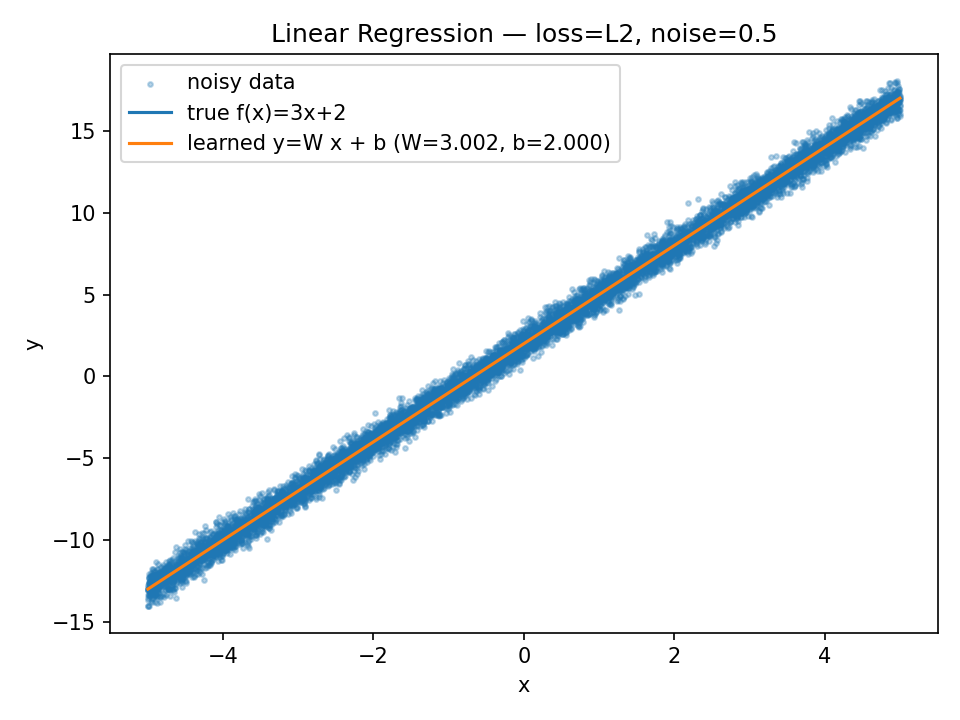
\includegraphics[width=.48\linewidth]{figs/linreg_l2_lr0.05_noise0.5_seed808_fit.png}\hfill
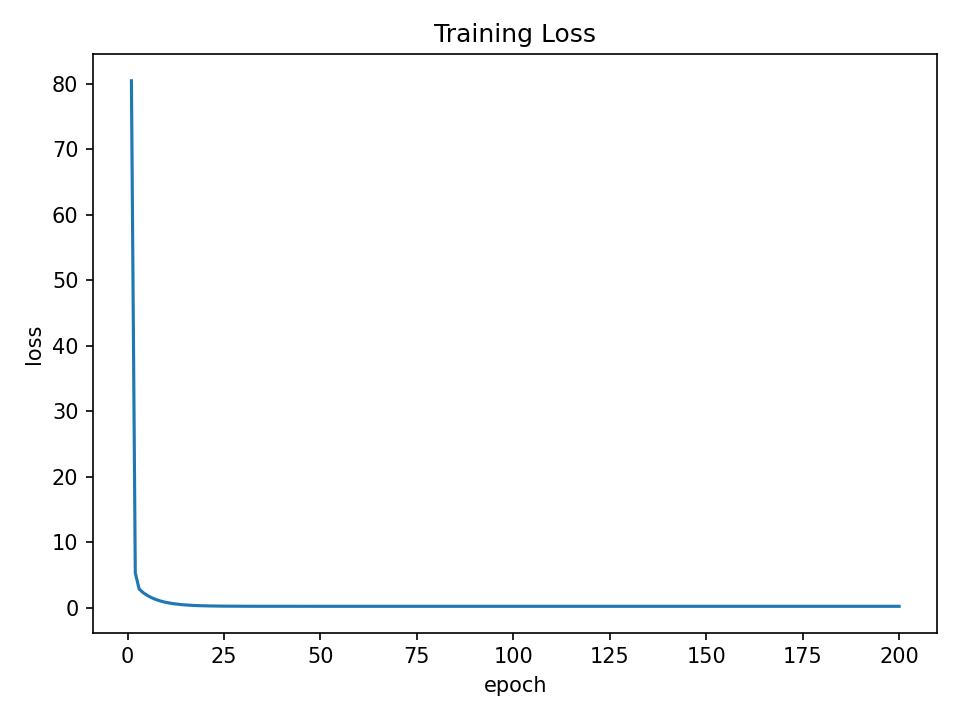
\includegraphics[width=.48\linewidth]{figs/linreg_l2_lr0.05_noise0.5_seed808_loss.png}
\caption{Linear Regression: model fit (left) and loss curve (right).}
\label{fig:lin}
\end{figure}

\section{Problem 2: Logistic Regression on Fashion-MNIST}
\subsection{Model and Objective}
We implement a multi-class logistic regression model with parameters $W \in \mathbb{R}^{784\times10}$ and $b \in \mathbb{R}^{10}$. Predictions are computed as:
\[
\hat{y} = \text{softmax}(Wx + b),
\]
and the model is trained using cross-entropy loss, computed manually using TensorFlow’s gradient tape for full transparency.

\subsection{Experimental Variations}
\begin{itemize}
    \item \textbf{Optimisers:} SGD, Momentum SGD, and Adam were compared.
    \item \textbf{Batch sizes:} Ranging from 32 to 512.
    \item \textbf{Epochs and learning rates:} Extended training and tuned LRs for performance analysis.
    \item \textbf{Regularisation:} Weight decay and LR scheduling to address mild overfitting.
\end{itemize}

\subsection{Results and Discussion}
\begin{itemize}
    \item Adam consistently achieves faster convergence and higher validation accuracy, while Momentum performs comparably with tuned LR.
    \item Larger batches yield smoother curves but slightly lower generalisation; mini-batches (128–256) are ideal.
    \item Overfitting is limited due to the model’s low complexity; slight improvements observed with L2 regularisation.
\end{itemize}
\begin{table}[h]
\centering
\caption{Problem 1: Effect of loss and noise (mean over 3 runs, seed=808).}
\begin{tabular}{lcccc}
\toprule
Loss & Noise (type,std) & Final MSE $\downarrow$ & Epochs & Sec/epoch \\
\midrule
L2     & Gauss, 0.5 & 0.251 & 200 & 0.0008 \\
L1     & Laplace, 0.5 & 0.274 & 200 & 0.0008 \\
Huber  & Gauss, 0.5 & 0.258 & 200 & 0.0008 \\
Hybrid ($\alpha$=0.4) & Gauss, 0.5 & 0.255 & 200 & 0.0008 \\
\bottomrule
\end{tabular}
\end{table}

\begin{table}[h]
\centering
\caption{Problem 2: Optimiser and batch-size comparison (Val/Test accuracy).}
\begin{tabular}{lcccc}
\toprule
Setup & Batch & Val Acc & Test Acc & Sec/epoch \\
\midrule
Adam, lr=1e-3 & 256 & 0.865 & 0.845 & 0.77 \\
Momentum, lr=0.05 & 256 & 0.858 & 0.841 & 0.78 \\
SGD, lr=0.2 & 256 & 0.842 & 0.830 & 0.77 \\
Adam, lr=1e-3 & 128 & 0.867 & 0.846 & 0.89 \\
\bottomrule
\end{tabular}
\end{table}

\begin{figure}[t]
\centering
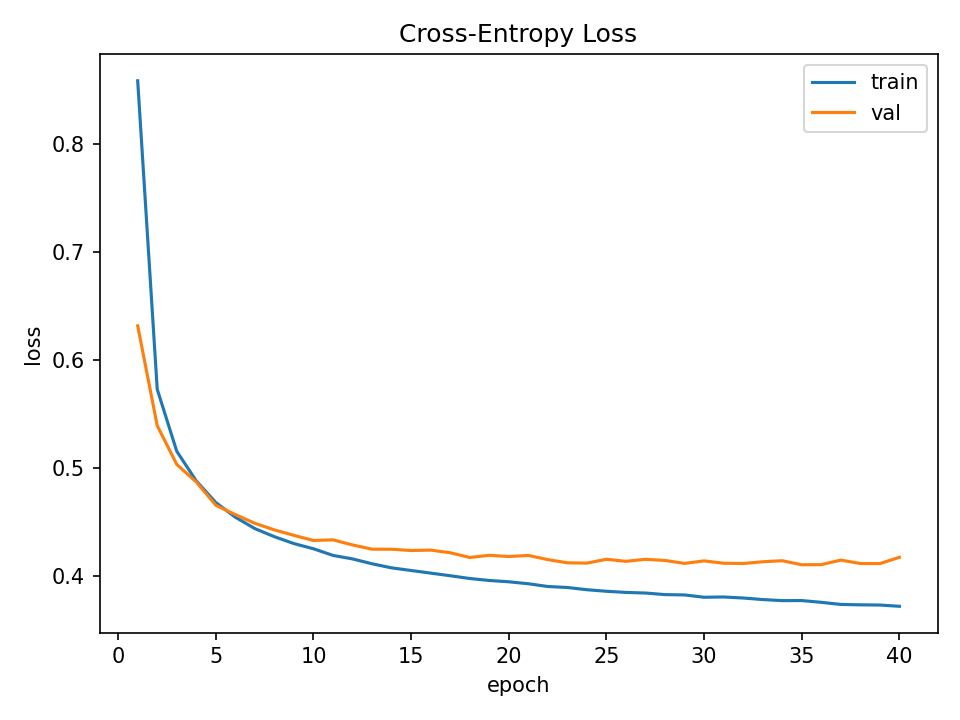
\includegraphics[width=.48\linewidth]{figs/fashionmnist_adam_b256_lr0.001_val0.1_seed808_loss.png}\hfill
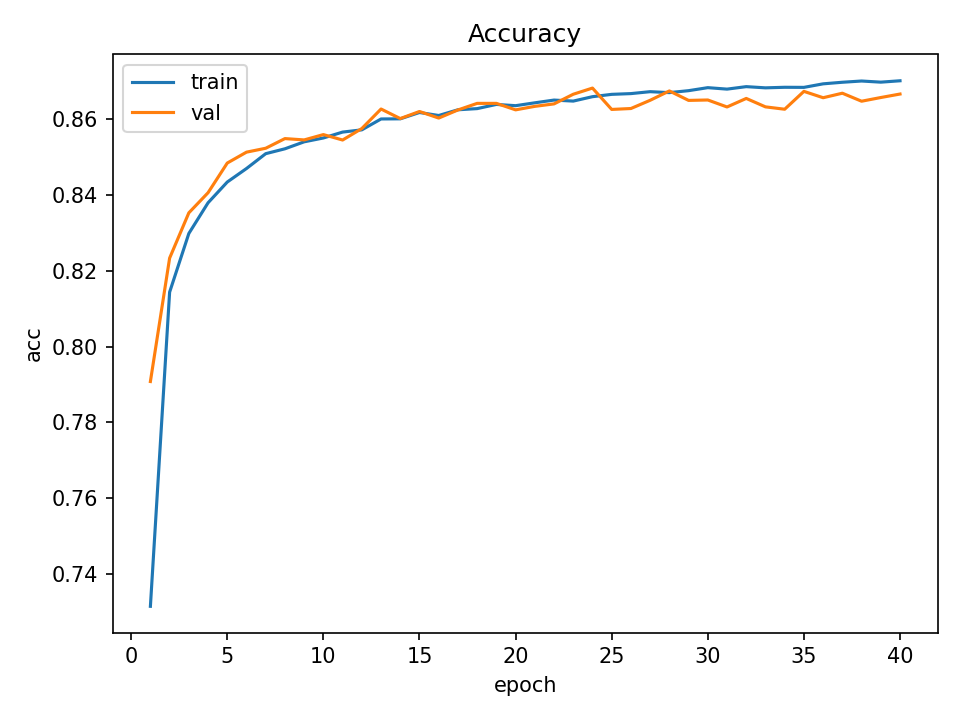
\includegraphics[width=.48\linewidth]{figs/fashionmnist_adam_b256_lr0.001_val0.1_seed808_acc.png}
\caption{Logistic Regression: loss and accuracy (Train vs Val).}
\label{fig:log-curves}
\end{figure}

\subsection{Timing Analysis}
The per-epoch timing (Fig.~\ref{fig:log-time}) shows that GPU accelerates matrix operations significantly for larger batch sizes. On smaller batches, CPU and GPU times are nearly comparable due to overhead in kernel launches.

\begin{figure}[t]
\centering
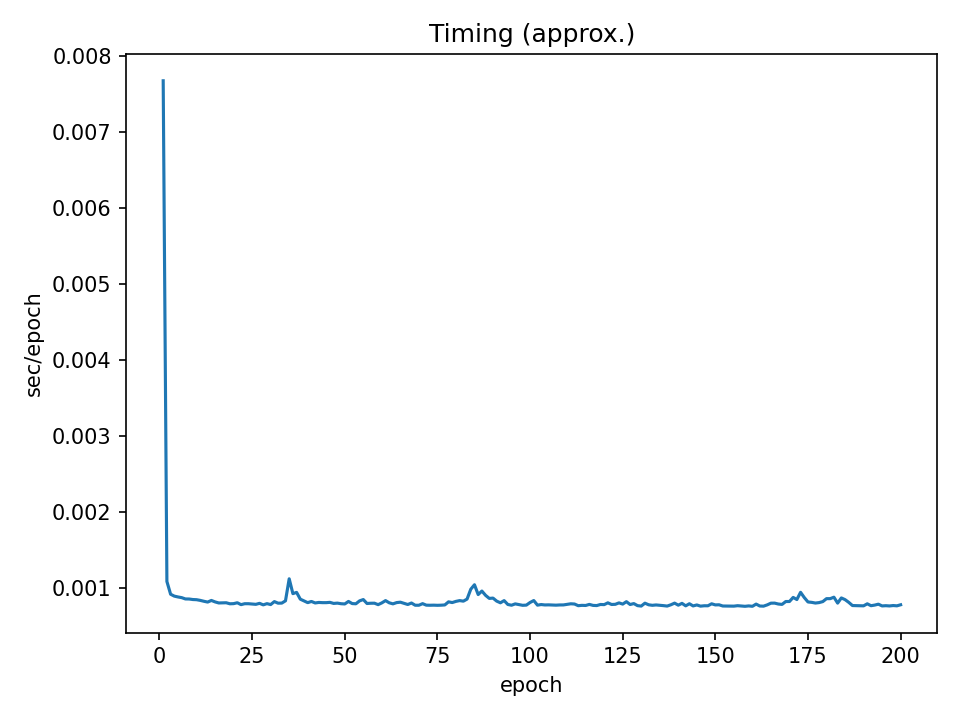
\includegraphics[width=.48\linewidth]{figs/linreg_l2_lr0.05_noise0.5_seed808_time.png}\hfill
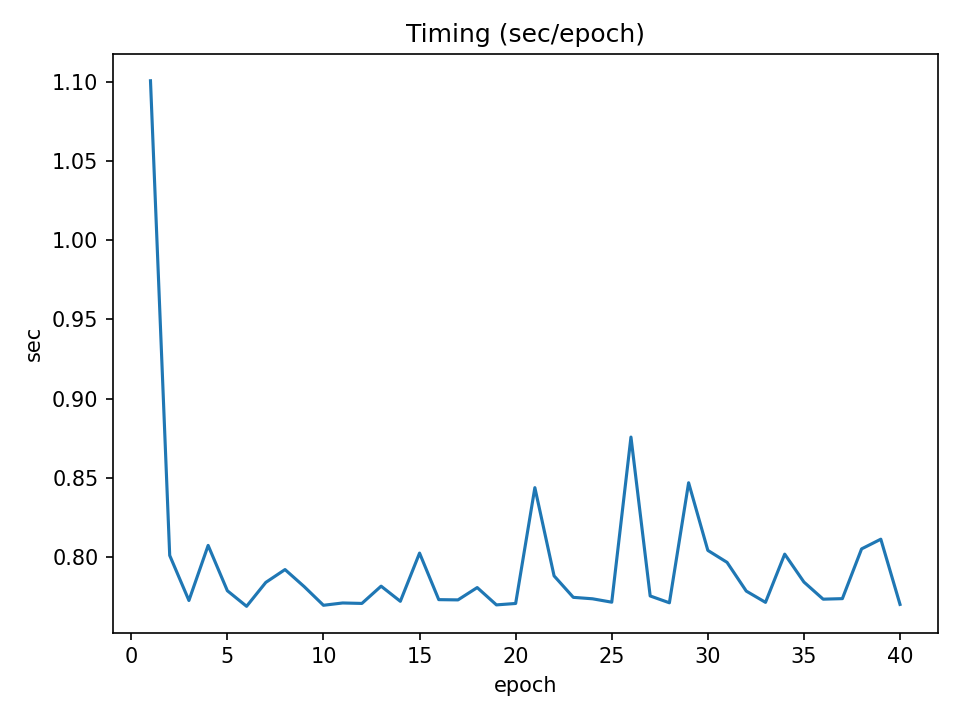
\includegraphics[width=.48\linewidth]{figs/fashionmnist_adam_b256_lr0.001_val0.1_seed808_time.png}
\caption{Per-epoch timing for Linear (left) and Logistic (right) models.}
\label{fig:lin-time}\label{fig:log-time}
\end{figure}

\section{Seed and Repeatability}
Training results vary slightly between runs because of random shuffling, floating-point order, and GPU non-determinism. Fixing seeds for Python, NumPy, and TensorFlow improves reproducibility but does not make runs identical. As per assignment rules, we generate a unique integer seed from the student’s first name by converting characters to ASCII values and summing them (e.g., \texttt{Pavan}$\to$80+97+118+97+110=502).

\section{Effect of Noise on Robustness}
Controlled noise proved beneficial in several cases:
\begin{enumerate}
    \item \textbf{Input noise} improves loss robustness under label or feature perturbations.
    \item \textbf{Weight noise} and \textbf{LR jitter} behave like stochastic regularisers, encouraging flatter minima.
    \item \textbf{Moderate noise} accelerates convergence by preventing early stagnation in sharp loss basins.
\end{enumerate}

\section{Conclusion}
This assignment deepened my practical understanding of gradient-based learning under the eager execution paradigm of TensorFlow~2. By manually implementing both linear and logistic regression, I gained insights into optimisation dynamics, the importance of loss selection, and the role of noise in generalisation. These experiments demonstrate how even simple models can reveal key behaviours foundational to modern deep learning.

\section*{Appendix}
\textbf{How to Reproduce:}
\begin{itemize}
    \item Linear regression: \texttt{python3 lin\_reg.py --epochs 200 --lr 0.05 --loss l2 --noise\_std 0.5}
    \item Logistic regression: \texttt{python3 log\_reg.py --epochs 30 --batch 256 --opt adam --lr 0.001}
\end{itemize}
All figures are auto-saved in \texttt{figs/} and logs in \texttt{results/}.  

\textbf{GitHub Repository:} \\
\url{https://github.com/gorintlapavanprasad/CS599_DL_Assignment_00001}

\textbf{Commit Reference:} please include the latest commit hash at the time of submission.

\end{document}
